\documentclass[12pt,letterpaper,spanish]{article}
\usepackage{pdfpages}
\usepackage[spanish]{babel}
\usepackage{multirow}
\usepackage{graphicx} % Required for inserting images
\usepackage{url}

\title{Modelo computacional para generar inferencias causales en sistemas de gestión de aprendizaje (LMS)}
\author{Víctor Ortiz-Pérez}
\date{June 2026}

\begin{document}
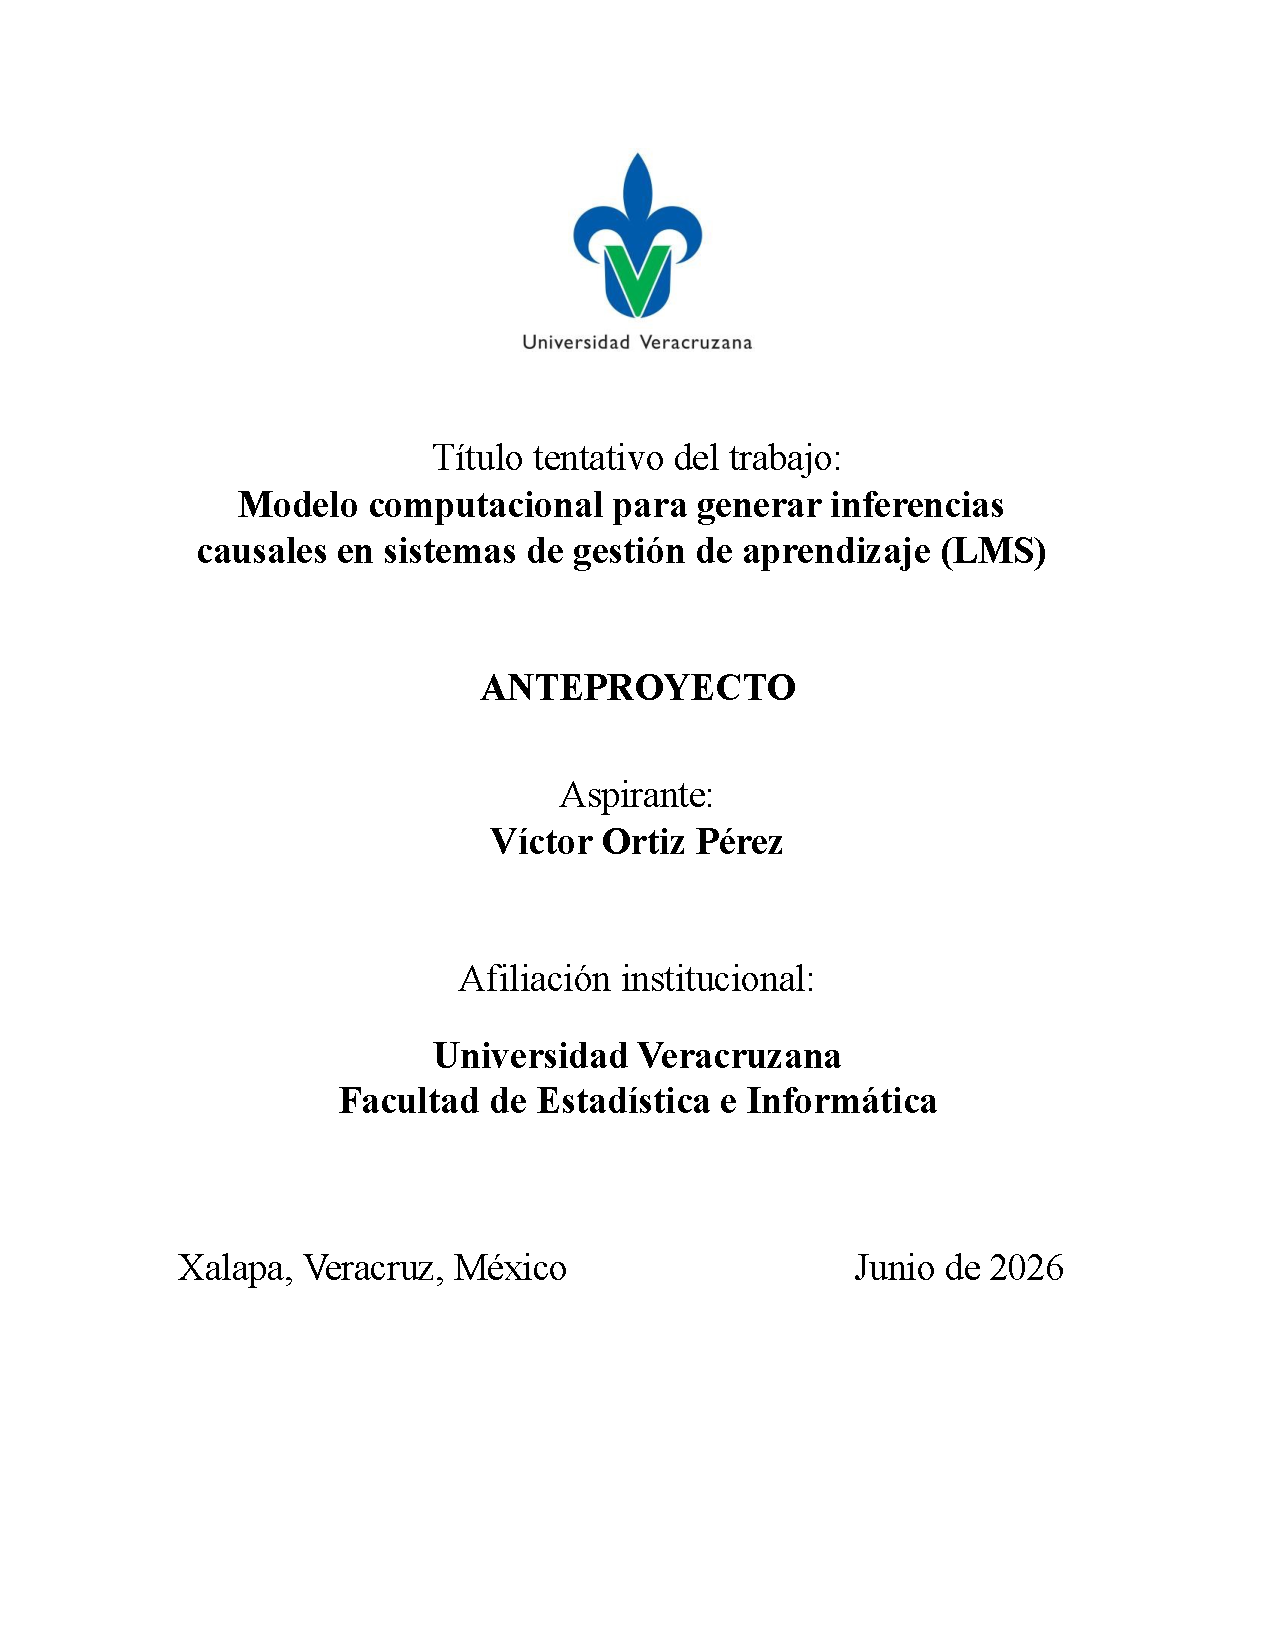
\includepdf{portada.pdf}
%\maketitle
\newpage
\tableofcontents
\newpage

\section{Introducción}
\subsection{Antecedentes}
En esta sección se presentan los antecedentes relevantes.
\subsection{Definición del problema}
\cite{nagai_analysis_2024}
\subsection{Justificación}
\subsection{Objetivo general}
\subsection{Objetivos específicos}
\begin{enumerate}
    \item Desarrollar un modelo computacional basado en técnicas de inteligencia artificial para generar inferencias causales en sistemas de gestión de aprendizaje (LMS).
    \item Evaluar la efectividad del modelo propuesto mediante la aplicación de casos de estudio en entornos educativos reales.
\end{enumerate}
\subsection{Hipótesis}
\newpage

\section{Metodología científica}
\subsection{Fases}
\subsection{Cronograma}
\subsection{Participantes}
\subsection{Instrumentos}
\subsection{Procedimiento y escenario}
\newpage

\section{Resultados}
\subsection{Análisis de resultados}
\subsection{Metas propuestas con la tesis}

\newpage
%Preguntar por qué en el ejemplo no tiene conclusiones, si es que no se necesitan o si se pueden incluir en esta sección.
\section{Conclusiones}

\newpage

\bibliographystyle{plain}
\bibliography{biblioai}

\end{document}